\documentclass[conference]{IEEEtran}
\IEEEoverridecommandlockouts
\usepackage{cite}
\usepackage{amsmath,amssymb}
\usepackage{graphicx}
\usepackage{booktabs}
\usepackage{multirow}
\usepackage{xcolor}
\usepackage{algorithm}
\usepackage{algpseudocode}
\usepackage{tikz}
\usetikzlibrary{arrows.meta,positioning,fit,calc}
\usepackage[hidelinks]{hyperref}
\usepackage{url}
\usepackage{balance}

\newcommand{\code}[1]{\texttt{\small #1}}

\begin{document}

\title{TrialSieve: Evidence-Grounded Criterion-Level Clinical-Trial Screening with a Fine-Tuned Small Transformer and From-Scratch Efficient Inference}

\author{\IEEEauthorblockN{Muhammad Ibrahim Malik (23i-0694)}
\IEEEauthorblockA{\textit{Department of Computer Science} \\
\textit{FAST-NUCES Islamabad}, Pakistan\\
Generative AI, Assignment 2 --- Instructor: Dr.\ Akhter Jamil}}

\maketitle

\begin{abstract}
Screening patients against the eligibility criteria of clinical trials is slow, manual work. We study whether a small, locally executable decoder Transformer can make criterion-level eligibility judgements and cite the patient-note sentences that support them. Using the TrialGPT Criterion Annotations dataset with a fixed patient-grouped split (37/8/8 patients), we fine-tune Qwen2.5-1.5B-Instruct with LoRA to emit a structured label and supporting sentence IDs. On the untouched test split (206 criteria) accuracy rises from 0.325 to 0.743, macro-F1 from 0.256 to 0.545 and evidence micro-F1 from 0.123 to 0.508. We re-implement the model's forward pass from its weights, with an explicit pre-allocated key/value cache, a tiled online-softmax attention kernel and greedy speculative decoding with a fine-tuned 0.5B draft model, and verify each against a reference path token-by-token. On a T4 GPU, KV caching gives up to 4.1$\times$ lower latency for 512-token prompts; tiled attention uses 13$\times$ less memory than explicit attention at 2048 tokens but runs 9$\times$ slower in pure PyTorch; speculative decoding is exact in all 72 runs but gains at most 1.07$\times$, while on a CPU, where decoding is bandwidth bound, it gains more. A batched ragged-cache decoder screens a 21-criterion trial 3.6$\times$ faster on a laptop CPU. Everything is exposed in a browser application that produces auditable screening reports. The system is an educational prototype, not a clinical decision tool.
\end{abstract}

\begin{IEEEkeywords}
clinical trial matching, eligibility screening, LoRA, KV cache, online softmax, speculative decoding, evidence extraction
\end{IEEEkeywords}

\section{Introduction and Problem Statement}
Clinical trials define who may enrol through free-text inclusion and exclusion criteria. Matching a patient record against dozens of criteria is labour-intensive, and recent work shows that large language models (LLMs) can assist by judging each criterion and explaining the decision~\cite{jin2024trialgpt,wornow2024zeroshot}. These systems rely on large proprietary models, which raises cost, privacy and reproducibility concerns for clinical text.

\textbf{Problem.} Given (i) a patient description split into numbered sentences, (ii) a criterion type (inclusion or exclusion) and (iii) the criterion text, predict the expert eligibility category, keeping the dataset's categories \emph{not enough information} and \emph{not applicable} rather than collapsing them into yes/no, and return the IDs of the patient sentences that support the decision. Absence of information must never be read as evidence of eligibility or ineligibility.

\textbf{Contributions.} (1) A LoRA-fine-tuned Qwen2.5-1.5B model that emits a structured label and sentence-ID evidence, evaluated before and after fine-tuning on a fixed, leakage-checked patient split. (2) A from-scratch Qwen2 forward pass with an explicit KV cache, including batched decoding of sequences with different cache lengths and prefix reuse across criteria. (3) A tiled online-softmax attention kernel. (4) Greedy speculative decoding with cache rollback. (5) An empirical analysis of when each mechanism helps on a T4 GPU and on a laptop CPU. (6) A browser application with auditable, downloadable reports.

\section{Related Work}
\textbf{LLM-based patient--trial matching.} Koopman and Zuccon~\cite{koopman2016test} released patient topics (the \code{sigir-*} patients in our data) and trial relevance judgements. TrialGPT~\cite{jin2024trialgpt} uses GPT-4 to predict criterion-level eligibility with explanations and cited sentences, then aggregates and ranks trials; its expert-annotated criterion predictions form our dataset. Wornow et al.~\cite{wornow2024zeroshot} show zero-shot GPT-4 matching on a cohort benchmark. Both depend on proprietary models; neither studies small open models under supervised adaptation, and their explanations are free text that is hard to verify. We instead require sentence IDs, which can be checked automatically, and use only a 1.5B-parameter open model.

\textbf{Open decoder models and parameter-efficient fine-tuning.} Qwen2/2.5~\cite{yang2024qwen2,qwen2.5} and Llama~3~\cite{dubey2024llama3} provide small instruction-tuned decoders built on the Transformer~\cite{vaswani2017attention} with rotary position embeddings (RoPE)~\cite{su2024roformer} and grouped-query attention (GQA)~\cite{ainslie2023gqa}. LoRA~\cite{hu2022lora} trains low-rank updates to frozen weights, and QLoRA~\cite{dettmers2023qlora} additionally quantises the base model to 4 bits. LoRA's limitation is a smaller update space than full fine-tuning; QLoRA's is quantisation error and dependence on CUDA-only kernels. Because a 1.5B model fits a 16\,GB T4 in fp16, we use plain LoRA and avoid quantisation error.

\textbf{Efficient inference.} Caching keys and values turns per-token decoding from re-processing the whole sequence into processing one token~\cite{pope2023scaling}; vLLM~\cite{kwon2023vllm} manages cache memory in pages. Our setting is single-user, so we pre-allocate a contiguous cache and add rollback and ragged batching. Online softmax~\cite{milakov2018online} computes softmax normalisers in one pass; Rabe and Staats~\cite{rabe2021selfattention} and FlashAttention~\cite{dao2022flashattention} use it to tile attention so the full score matrix is never stored. FlashAttention's speed comes from a fused, IO-aware CUDA kernel, which an educational PyTorch loop cannot match; we measure that gap. Speculative decoding~\cite{leviathan2023speculative,chen2023speculative} lets a small draft model propose tokens that the target verifies in one pass, giving identical greedy output. The reported speed-ups assume the target pass is much more expensive than the draft pass; we test that assumption on two kinds of hardware.

\section{Materials and Methods}
\subsection{Dataset and Patient-Grouped Split}
We use only \code{ncbi/TrialGPT-Criterion-Annotations}: 1015 criterion annotations over 53 patients and 103 trials. Each row has the patient note (already split into numbered sentences, 3--14 per note, about 100 words), criterion type and text, the expert label and the expert evidence sentences. The four GPT-4 columns (explanation, its correctness, sentences and label) are dropped when the split files are written and are never used. One row has an empty criterion text; it is kept as an empty string. 610 rows (60\%) have no expert evidence sentences.

Following the protocol, unique patient IDs are sorted, shuffled with \code{numpy.random.default\_rng(42)} and assigned 37/8/8 to train/validation/test. The script asserts that the three patient sets are disjoint and that every annotation appears in exactly one split, and writes a manifest with patient IDs and counts (Table~\ref{tab:split}). The test split contains no \emph{excluded} example, so that class cannot be scored on test. Prompts and checkpoints were chosen on validation only; the test split was evaluated once, after the model, prompt and decoding settings were frozen.

\begin{table}[t]
\caption{Patient-grouped split (expert labels).}
\label{tab:split}
\centering\footnotesize
\begin{tabular}{@{}lrrrrrrrr@{}}
\toprule
Split & Pat. & Ann. & inc & n.inc & exc & n.exc & NEI & N/A\\
\midrule
Train & 37 & 603 & 88 & 13 & 8 & 292 & 174 & 28\\
Val & 8 & 206 & 35 & 3 & 2 & 101 & 53 & 12\\
Test & 8 & 206 & 27 & 7 & 0 & 91 & 66 & 15\\
\bottomrule
\end{tabular}
\end{table}

\subsection{Model Selection}
Table~\ref{tab:models} compares the candidates. The deciding constraints were: training on a free 16\,GB T4 without quantisation; CPU inference on a 16\,GB-RAM laptop for the live demonstration; a smaller model with the \emph{same tokenizer} as a speculative draft; and a permissive licence. Qwen2.5-1.5B-Instruct meets all four: 1.54B parameters (3.1\,GB in fp16, 6.2\,GB in fp32), Apache-2.0, a 32k context that easily covers our prompts (at most 650 tokens), and Qwen2.5-0.5B-Instruct shares its 151,936-entry vocabulary. Its GQA layout (12 query heads, 2 KV heads, head dimension 128, 28 layers) makes the KV cache small: $2\times 28\times 2\times 128\times 2$\,B $=28$\,KiB per token in fp16, six times less than with full multi-head attention. We rejected Llama-3.2-1B because it requires gated access under a custom licence and its only same-tokenizer sibling (3B) is too slow for CPU demonstrations. Qwen2.5-3B would need QLoRA on a T4 and runs at under 1 token/s on our laptop.

\begin{table}[t]
\caption{Candidate open-weight decoders (public model cards; memory = weights only).}
\label{tab:models}
\centering\footnotesize
\setlength{\tabcolsep}{3pt}
\begin{tabular}{@{}lrrrrll@{}}
\toprule
Model & Params & Layers & Q/KV heads & fp16 & Licence & Role\\
\midrule
Qwen2.5-1.5B-Instr. & 1.54B & 28 & 12/2 & 3.1\,GB & Apache-2.0 & \textbf{target}\\
Qwen2.5-0.5B-Instr. & 0.49B & 24 & 14/2 & 1.0\,GB & Apache-2.0 & \textbf{draft}\\
Qwen2.5-3B-Instr. & 3.09B & 36 & 16/2 & 6.2\,GB & Qwen research & rejected\\
Llama-3.2-1B-Instr. & 1.24B & 16 & 32/8 & 2.5\,GB & Llama 3.2 (gated) & rejected\\
Llama-3.2-3B-Instr. & 3.21B & 28 & 24/8 & 6.4\,GB & Llama 3.2 (gated) & rejected\\
\bottomrule
\end{tabular}
\end{table}

\subsection{Input/Output Format and Tokenization}
Each example becomes a chat prompt: a system message stating that only information in the note may be used and that absence of information is not evidence; then the numbered note, the criterion type, the criterion text, the four allowed labels for that type with one-line definitions, and the required JSON schema. The target is
\code{\{"label": "<label>", "evidence\_sentence\_ids": [IDs]\}}, followed by the end-of-turn token. Outputs are parsed by extracting the first JSON object. A label outside the criterion type's label set becomes \emph{invalid output} and counts as an error; it is never silently mapped to another class. Evidence IDs outside the note are discarded.
Prompts tokenized with the Qwen chat template have 357/369/340 tokens on average (train/val/test) and at most 650. The training sequence limit is 1024 tokens, so \textbf{no example is truncated} (verified and logged). If truncation were needed, the script would trim the prompt from the left and never the answer, which could remove early note sentences. This is why it is logged.

\subsection{Fine-Tuning}
We apply LoRA (rank 16, $\alpha=32$, dropout 0.05) to all attention and MLP projections (q, k, v, o, gate, up, down), which is 18.5M trainable parameters (1.18\%). The objective is next-token cross-entropy on the answer tokens only; prompt tokens are masked with $-100$. We train for 3 epochs with AdamW, learning rate $2\times10^{-4}$, cosine schedule with 5\% warm-up, micro-batch 2 with gradient accumulation 8 (effective batch 16, 114 steps), fp16 mixed precision, gradient checkpointing and seed 42. A first attempt with micro-batch 4 ran out of memory on the T4: with a 151,936-token vocabulary the fp32 logits alone take about 1.6\,GB per batch. Validation loss is computed every 10 steps, and the best checkpoint (step 80, validation loss 0.113) is kept. Training took 15.8 minutes on one T4 (Fig.~\ref{fig:training}). The 0.5B draft is fine-tuned the same way (8.8M LoRA parameters, 8.0 minutes) so that its proposals follow the target's output format. The adapter and logs are published on Hugging Face.

\begin{figure}[t]
\centering
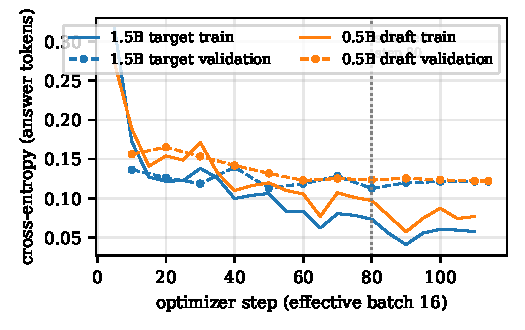
\includegraphics[width=\columnwidth]{figures/training.pdf}
\caption{Training and validation loss. Validation loss flattens after step 80 while training loss keeps falling (beginning of overfitting); the step-80 checkpoint is selected by validation loss.}
\label{fig:training}
\end{figure}

\subsection{System Architecture}
Fig.~\ref{fig:arch} shows the pipeline. Only the weights come from Hugging Face. The forward pass, cache, attention kernels and decoding loops are our own code (\code{src/trialsieve}).

\begin{figure*}[t]
\centering
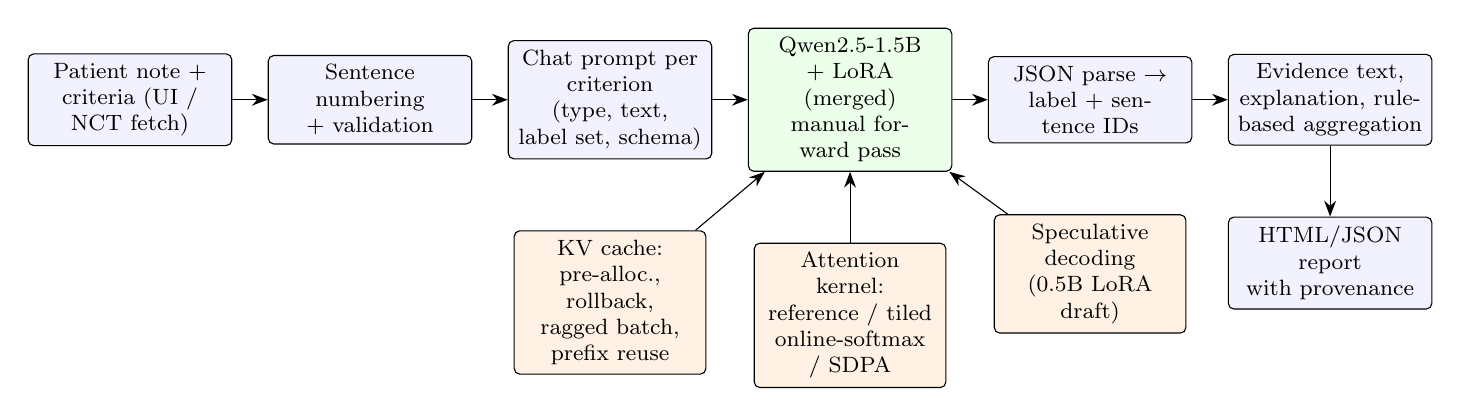
\begin{tikzpicture}[font=\footnotesize, node distance=0.35cm and 0.45cm,
  box/.style={draw, rounded corners=2pt, align=center, fill=blue!5, minimum height=0.9cm, text width=2.35cm},
  mod/.style={draw, rounded corners=2pt, align=center, fill=orange!10, minimum height=0.75cm, text width=2.2cm},
  arr/.style={-{Stealth[length=2mm]}}]
\node[box] (in) {Patient note +\\ criteria (UI / NCT fetch)};
\node[box, right=of in] (num) {Sentence numbering\\ + validation};
\node[box, right=of num] (prompt) {Chat prompt per\\ criterion (type, text,\\ label set, schema)};
\node[box, right=of prompt, fill=green!8] (model) {Qwen2.5-1.5B\\ + LoRA (merged)\\ manual forward pass};
\node[box, right=of model] (parse) {JSON parse $\rightarrow$\\ label + sentence IDs};
\node[box, right=of parse] (agg) {Evidence text,\\ explanation, rule-\\ based aggregation};
\node[box, below=0.9cm of agg] (rep) {HTML/JSON report\\ with provenance};
\node[mod, below=0.9cm of prompt] (kv) {KV cache: pre-alloc.,\\ rollback, ragged batch,\\ prefix reuse};
\node[mod, below=0.9cm of model] (att) {Attention kernel:\\ reference / tiled\\ online-softmax / SDPA};
\node[mod, below=0.9cm of parse] (spec) {Speculative decoding\\ (0.5B LoRA draft)};
\draw[arr] (in) -- (num); \draw[arr] (num) -- (prompt); \draw[arr] (prompt) -- (model);
\draw[arr] (model) -- (parse); \draw[arr] (parse) -- (agg); \draw[arr] (agg) -- (rep);
\draw[arr] (kv) -- (model); \draw[arr] (att) -- (model); \draw[arr] (spec) -- (model);
\end{tikzpicture}
\caption{TrialSieve pipeline. Orange modules are implemented from scratch and can be switched at run time in the application.}
\label{fig:arch}
\end{figure*}

\subsection{Manual Forward Pass and KV Cache}
For new tokens at absolute positions $p_0,\dots,p_0+T-1$, each layer computes $x=\mathrm{RMSNorm}(h)$, $q,k,v$ projections (with biases), RoPE with $\theta=10^6$ applied to $q$ and $k$ at their absolute positions, attention, an output projection and residual, then a SwiGLU MLP and residual. The cache stores \emph{post-RoPE} keys and values in pre-allocated tensors $K,V\in\mathbb{R}^{L\times B\times H_{kv}\times N_{max}\times d}$ with a length counter $n$. A forward call writes new keys/values to slots $[n, n+T)$, attends over slots $[0,n+T)$ and advances $n$. Position handling therefore reduces to one rule: query $i$ of the call sits at position $n+i$ and may attend to key $j$ iff $j\le n+i$. The same rule covers prefill ($n=0$), single-token decoding ($T=1$) and multi-token speculative verification. Each of the 2 KV heads is shared by 6 query heads (GQA). Rolling back after rejected speculative tokens only lowers $n$; stale slots are never read and are later overwritten. The uncached reference path re-runs the entire sequence at every step without any state.

\textbf{Prefix reuse and ragged batching.} All criteria for one patient share the system prompt and note (238 tokens in our example). (i) Sequential prefix reuse keeps the previous cache, rolls it back to the longest common token prefix with the next prompt and prefills only the remainder. (ii) Batched decoding prefills the shared prefix once, copies it into every row of a batched cache, prefills all criterion suffixes together right-padded (causal masking guarantees that real tokens never see the padding after them), then decodes all rows together. Each row $b$ keeps its own length $n_b$: its new key is scattered to slot $n_b$, RoPE uses position $n_b$, and a per-row mask allows keys $0..n_b$ only. On CPU a decoding step is memory-bandwidth bound, so $B$ rows cost little more than one.

\subsection{Reference and Tiled Online-Softmax Attention}
The reference computes $S=QK^\top/\sqrt{d}$ in fp32, applies the causal (and optional per-row) mask with $-\infty$, subtracts the row maximum and normalises. The tiled kernel (Algorithm~\ref{alg:tiled}) processes query blocks and streams key/value blocks, keeping per query row a running maximum $m$, normaliser $\ell$ and unnormalised output $a$~\cite{milakov2018online,dao2022flashattention}. Key blocks entirely in the causal future are skipped, and masking is applied only to blocks that straddle the diagonal. Rows with no visible key so far keep $m=-\infty$; we substitute 0 in the exponent to avoid $\infty-\infty$.

\begin{algorithm}[t]
\caption{Tiled causal attention with online softmax}
\label{alg:tiled}
\footnotesize
\begin{algorithmic}[1]
\For{each query block $Q_i$ (positions $P_i$)}
  \State $m\gets-\infty,\ \ell\gets 0,\ a\gets 0$
  \For{each key block $K_j,V_j$ with $\min(\mathrm{pos}(K_j))\le\max(P_i)$}
    \State $S\gets Q_iK_j^\top/\sqrt d$;\ mask $S$ where key pos $>$ query pos
    \State $m'\gets\max(m,\mathrm{rowmax}(S))$;\ $c\gets e^{m-m'}$;\ $E\gets e^{S-m'}$
    \State $\ell\gets c\,\ell+\mathrm{rowsum}(E)$;\ $a\gets c\,a+EV_j$;\ $m\gets m'$
  \EndFor
  \State $O_i\gets a/\ell$
\EndFor
\end{algorithmic}
\end{algorithm}

\subsection{Greedy Speculative Decoding}
Algorithm~\ref{alg:spec} keeps the invariant that the target cache holds every committed token except the newest. Each round, the draft catches up on committed tokens it has not cached and proposes $k$ tokens greedily. The target scores $[x_{last}, d_1..d_k]$ in one pass, which gives its own greedy choice $t_1..t_{k+1}$ after each prefix. The longest prefix with $d_i=t_i$ is accepted, then $t_{n+1}$ is appended (a correction, or a free bonus token when all $k$ match). Both caches are rolled back to drop rejected tokens. By construction the output equals greedy decoding of the target; we verify this rather than assume it.

\begin{algorithm}[t]
\caption{Greedy speculative decoding with cache rollback}
\label{alg:spec}
\footnotesize
\begin{algorithmic}[1]
\State target prefill on prompt $\rightarrow$ first token; $s\gets$ prompt $+$ [first]
\While{not EOS and $|out|<N$}
  \State draft: feed $s[n_{draft}:]$, then propose $d_1..d_k$ greedily
  \State $t_{1..k+1}\gets\arg\max$ target$([s_{-1},d_1..d_k])$ \Comment{one pass}
  \State $n\gets$ largest $n$ with $d_{1..n}=t_{1..n}$;\ $s\mathrel{+}=d_{1..n}\,\|\,t_{n+1}$
  \State target.rollback$(|s|-1)$;\ draft.rollback$(\min(n_{draft},|s|-1))$
\EndWhile
\end{algorithmic}
\end{algorithm}

\subsection{Application Workflow}
The Gradio application (started by double-clicking \code{run\_app.bat}; it works offline once the models are cached) accepts a free-text note, which is split into numbered sentences automatically. Inclusion and exclusion criteria can be typed, loaded from a validation example, or fetched from the public ClinicalTrials.gov API by NCT ID. For each criterion it shows the label, cited sentence IDs and their text, and an explanation built \emph{only} from the cited sentences. A \emph{not enough information} result is explicitly reported as missing information rather than as evidence. The overall outcome is an explicit rule, not a model output, because the dataset has no trial-level ground truth: \emph{likely ineligible} if any inclusion criterion is \emph{not included} or any exclusion criterion is \emph{excluded}; otherwise \emph{needs review} if any criterion is undecidable or invalid; otherwise \emph{potentially eligible}. \emph{Not applicable} criteria are ignored. Input validation rejects empty notes, notes over 1200 tokens, more than 40 criteria or over-long criteria with a message instead of crashing. Reports are downloadable as HTML and JSON with provenance: UTC time, code commit, model and adapter IDs, decoding and attention settings, an input SHA-256 fingerprint and runtime. Every page carries the notice that this is an educational screening prototype. Users can switch live between the fine-tuned and base model (the LoRA update is unmerged and disabled in place), any decoding mode and any attention kernel. An inference lab runs the same prompt through each decoder and reports token identity, prefill/decode time, throughput, acceptance rate and cache size.

\section{Experimental Setup and Metrics}
\textbf{Hardware.} Training and GPU benchmarks: Kaggle, one NVIDIA T4 (16\,GB), PyTorch 2.11, fp16. Application and CPU benchmarks: laptop with an Intel Core i7-1255U (2 performance + 8 efficiency cores), 16\,GB RAM, fp32.

\textbf{Decoding.} All evaluations use greedy decoding with at most 64 new tokens. Qwen's default generation configuration silently applies a repetition penalty of 1.1 even when sampling is off. We found this when our cached decoder disagreed with \code{generate()} while matching the model's own forward pass. We therefore override it to 1.0 everywhere, so all reported numbers are pure greedy decoding and directly comparable with our decoders.

\textbf{Classification metrics.} Accuracy; macro-F1 over the classes that occur in the gold labels of the evaluated subset (so the absent \emph{excluded} class does not count as an automatic zero on test); per-class precision/recall/F1; and confusion matrices, overall and separately for inclusion and exclusion criteria.

\textbf{Evidence metrics.} Micro precision/recall/F1 pool TP/FP/FN of sentence IDs over all records. Macro scores average per-record P/R/F1 with explicit conventions for empty sets: gold and prediction both empty $\Rightarrow$ P=R=F1=1 (correctly cited nothing); gold empty, prediction non-empty $\Rightarrow$ P=0, R=1, F1=0; gold non-empty, prediction empty $\Rightarrow$ P=1, R=0, F1=0. Because 60\% of records have no gold evidence, the macro average is inflated by empty-empty agreement, so we also report it restricted to records with non-empty gold evidence. We regard micro-F1 and this restricted score as the honest measures.

\textbf{Benchmark protocol.} Every timed configuration gets one untimed warm-up run, then three timed runs. On GPU the timer calls \code{torch.cuda.synchronize()} before and after, and we report the median. Peak memory is the CUDA allocator peak above the memory already in use (weights excluded). KV benchmarks use fixed output lengths (EOS ignored) on synthetic clinical prompts of 64/256/512 tokens. Speculative and attention end-to-end benchmarks use 10 validation prompts plus 2 free-text prompts, so the test split is never used for tuning.

\section{Results and Discussion}
\subsection{Before vs.\ After Fine-Tuning}
Table~\ref{tab:main} compares the same model, prompt and greedy decoding before and after fine-tuning on identical examples. Fine-tuning more than doubles accuracy on both splits, and the validation and test results agree closely (0.733 vs.\ 0.743), so no tuning overfitted validation. The base model's main failure is predicting \emph{not applicable} for most criteria (101 of 206 validation predictions), and it rarely cites the right sentences (evidence micro precision 0.079 on test). After fine-tuning, invalid outputs drop to zero, and the model reproduces the output format and the dataset's label conventions.

\begin{table}[t]
\caption{Criterion-level results, base vs.\ LoRA (greedy, same prompt). Ev.\ = evidence; ne = gold non-empty.}
\label{tab:main}
\centering\footnotesize
\setlength{\tabcolsep}{3pt}
\begin{tabular}{@{}llrrrrr@{}}
\toprule
Split & Model / subset & Acc & Macro-F1 & Ev.\ $\mu$F1 & Ev.\ MF1 & Ev.\ F1$_{ne}$\\
\midrule
\multirow{2}{*}{Val} & Base, all & 0.345 & 0.221 & 0.124 & 0.336 & 0.168\\
 & LoRA, all & \textbf{0.733} & \textbf{0.431} & \textbf{0.522} & \textbf{0.729} & \textbf{0.535}\\
\midrule
\multirow{6}{*}{Test} & Base, all & 0.325 & 0.256 & 0.123 & 0.484 & 0.111\\
 & Base, inclusion & 0.160 & 0.149 & 0.235 & 0.449 & 0.081\\
 & Base, exclusion & 0.420 & 0.291 & 0.088 & 0.505 & 0.195\\
 & LoRA, all & \textbf{0.743} & \textbf{0.545} & \textbf{0.508} & \textbf{0.813} & \textbf{0.533}\\
 & LoRA, inclusion & 0.787 & 0.424 & 0.594 & 0.670 & 0.671\\
 & LoRA, exclusion & 0.718 & 0.433 & 0.158 & 0.895 & 0.143\\
\bottomrule
\end{tabular}
\end{table}

\begin{figure*}[t]
\centering
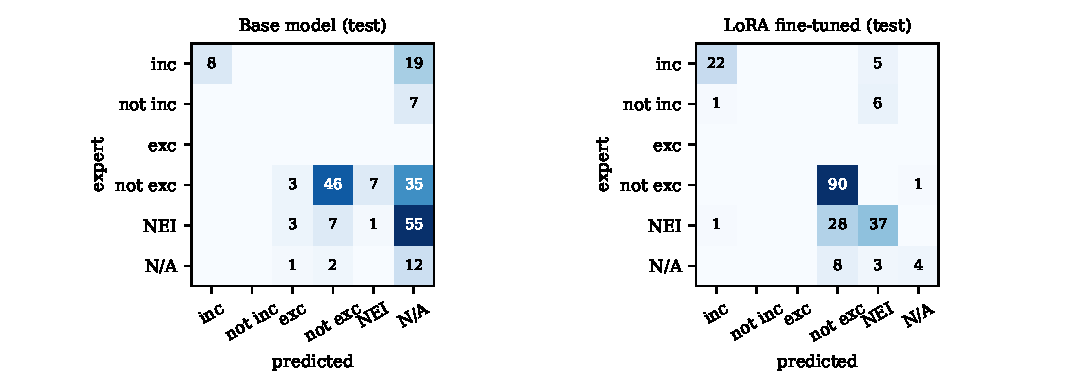
\includegraphics[width=0.82\textwidth]{figures/confusion.pdf}
\caption{Test confusion matrices (rows: expert, columns: predicted; NEI = not enough information, N/A = not applicable). The base model defaults to N/A; the fine-tuned model's dominant error is NEI$\rightarrow$not excluded.}
\label{fig:cm}
\end{figure*}

\subsection{Per-Class Behaviour}
On test (Fig.~\ref{fig:cm}), the fine-tuned model is strong on \emph{included} (P 0.92, R 0.82, F1 0.86) and \emph{not excluded} (P 0.71, R 0.99, F1 0.83), moderate on \emph{not enough information} (F1 0.63) and weak on \emph{not applicable} (F1 0.40, recall 0.27). It never predicts \emph{not included} (0/7). With only 13 training examples, and 8 for \emph{excluded}, these minority classes are not learned. That is the main reason macro-F1 (0.545) lags accuracy. Class re-weighting or oversampling is the obvious next step, but we did not tune it, to keep the test protocol clean within the time budget.

\subsection{Evidence Localisation}
Evidence quality differs sharply by criterion type. For inclusion criteria, micro-F1 is 0.594 (recall 0.74). For exclusion criteria, recall is only 0.094: the model usually answers \emph{not excluded} without citing anything, while experts often cite the sentence that rules the exclusion out (e.g.\ the age sentence for ``less than 18 years''). The empty-set convention matters a great deal. Exclusion macro-F1 is 0.895 because most exclusion records have empty gold \emph{and} empty predicted evidence, whereas F1 on records with gold evidence is 0.143. We therefore do not treat the macro score as evidence of good localisation.

\subsection{Error Analysis}
A rule-based taxonomy (\code{scripts/error\_analysis.py}) assigns every test prediction to the first matching category (Table~\ref{tab:errors}). Representative cases, identified by annotation ID:
\begin{enumerate}
\item \textbf{Missing information read as negative} (\#169, \#174, 28 cases): ``eGFR $<$30'' and ``previous axillary surgery'' are not mentioned; experts say \emph{not enough information}, the model says \emph{not excluded}. This is the most frequent error and exactly the failure the task warns about: absence treated as a negative finding. It mirrors a training-label asymmetry (292 \emph{not excluded} vs.\ 174 NEI).
\item \textbf{Contradictory evidence} (\#161, \#162, 6 cases): for ``patients undergoing elective carotid endarterectomy'' the note describes a cardiac catheterisation. Experts say \emph{not included}; the model answers \emph{not enough information} while citing sentences 0--2, which actually decide the criterion.
\item \textbf{Under-confident} (\#176): ``no history of central venous catheterisation'' for a patient who had femoral \emph{arterial} catheterisation. Experts say \emph{included} citing sentence 0; the model says NEI. Distinguishing arterial from venous access requires domain knowledge.
\item \textbf{Missed not-applicable} (\#422, 11 cases): ``if female, using birth control'' for a girl with no sexual partners. Experts say \emph{not applicable} (sentence 3); the model says NEI.
\item \textbf{Label ambiguity} (\#322): a pregnancy/contraception exclusion for a 48-year-old man. The model predicts \emph{not applicable}; experts chose \emph{not excluded}. Both are defensible, which suggests that part of the N/A error is annotation ambiguity rather than model failure.
\item \textbf{Over-commitment} (\#678): mild sleep-disordered breathing requires snoring on $\ge$3 nights/week for $\ge$3 months. The note says ``nighttime snoring'' without frequency or duration. Experts say NEI; the model says \emph{included} (same evidence sentence).
\item \textbf{Opposite decision} (\#164): ``surgical lower-limb revascularisation'' is predicted \emph{included} from a groin pseudo-aneurysm after catheterisation, citing sentences 0 and 2. The cited text is relevant but does not support the conclusion: an unsupported inference.
\item \textbf{Correct label, unsupported} (\#196, 13 cases): ``less than 18 years of age'' for a 40-year-old is correctly \emph{not excluded}, but no sentence is cited although sentence 0 states the age.
\item \textbf{Correct label, over-citation} (\#307, 15 cases): a long, complex inclusion criterion is correctly NEI, but the model cites all five sentences where experts cite one, lowering evidence precision.
\end{enumerate}
In the application, every one of these cases is traceable: each row links its label to the cited sentence text, and a NEI result lists the criterion under ``missing information'' instead of counting for or against the patient.

\begin{table}[t]
\caption{Error taxonomy on the test split (fine-tuned model, 206 criteria; first matching rule).}
\label{tab:errors}
\centering\footnotesize
\begin{tabular}{@{}lr@{}}
\toprule
Category & Count\\
\midrule
Missing information read as a negative finding (NEI$\rightarrow$not exc./not inc.) & 28\\
Missed \emph{not applicable} & 11\\
Cited evidence yet answered NEI (contradictory) & 6\\
Answered NEI although note decides the criterion & 5\\
Decided a criterion experts judged undecidable & 1\\
Opposite decision / other label error & 2\\
\midrule
Correct label, no evidence where experts cited some & 13\\
Correct label, cited sentences experts did not & 15\\
Correct label, missed some expert evidence & 2\\
\bottomrule
\end{tabular}
\end{table}

\subsection{KV-Cached Decoding}
\textbf{Correctness.} Our forward pass matches Hugging Face logits to within $3\times10^{-5}$ (fp32) with every attention kernel, both uncached and when the input is fed in arbitrary chunks through the cache. Under greedy decoding, cached, uncached and \code{generate()} outputs are token-identical in unit tests at three prompt/output lengths (fp32). This includes a 64-token-prompt case, prefix reuse, and ragged batching with all three kernels.

\textbf{Mismatch investigation.} On the T4 in fp16, 7 of 9 configurations are token-identical. The two exceptions (prompt 64, 64 and 128 new tokens) both diverge at token 20. Re-running that prompt in fp32 shows cached and uncached paths agree on all tokens, and at step 20 the top two candidates (`` and'' vs.\ ``,'') differ by only 0.0003 in a logit of about 26. fp16 has a resolution of about 0.016 at that magnitude, so the different summation orders of the two paths (one query over a cache vs.\ a full causal pass) flip the argmax. The mismatch is a numerical near-tie, not a cache bug.

\textbf{Performance.} Table~\ref{tab:kv} and Fig.~\ref{fig:kv} show that the benefit grows with context. Without a cache, decode throughput falls from 22.9 to 5.7 tokens/s as the prompt grows from 64 to 512 tokens, because every step re-processes the whole sequence. With the cache it stays at about 24 tokens/s, and latency improves 3.4--4.1$\times$ at 512 tokens. At 64 tokens the gain is only 2--8\%: a batch-1 step of a 1.5B model on a T4 is dominated by kernel-launch and Python overhead (28 layers $\times$ many small kernels), not arithmetic, so recomputing 64 extra tokens costs almost nothing. Peak extra memory is slightly \emph{higher} with the cache for short outputs, because the cache is pre-allocated for the full prompt+output length, and lower for long ones, where the uncached path's activations over the full sequence dominate. Analytically, the cache grows by 28\,KiB per token in fp16.

\begin{table}[t]
\caption{KV cache vs.\ no cache on a T4 (fp16, median of 3). Mem = peak memory above weights (MiB).}
\label{tab:kv}
\centering\footnotesize
\setlength{\tabcolsep}{3.5pt}
\begin{tabular}{@{}rrcrrrrr@{}}
\toprule
Prompt & New & Equal & No-cache s & KV s & Speed-up & Mem$_{nc}$ & Mem$_{kv}$\\
\midrule
64 & 16 & \checkmark & 0.70 & 0.68 & 1.02 & 6.7 & 9.9\\
64 & 64 & @20 & 2.80 & 2.71 & 1.03 & 11.2 & 9.9\\
64 & 128 & @20 & 5.79 & 5.37 & 1.08 & 14.7 & 12.3\\
256 & 16 & \checkmark & 1.26 & 0.67 & 1.88 & 18.8 & 25.3\\
256 & 64 & \checkmark & 5.40 & 2.69 & 2.01 & 22.1 & 26.5\\
256 & 128 & \checkmark & 11.10 & 5.33 & 2.08 & 30.9 & 28.3\\
512 & 16 & \checkmark & 2.51 & 0.75 & 3.36 & 48.9 & 61.2\\
512 & 64 & \checkmark & 10.58 & 2.73 & 3.88 & 56.2 & 62.5\\
512 & 128 & \checkmark & 22.29 & 5.39 & 4.14 & 68.3 & 64.3\\
\bottomrule
\end{tabular}
\end{table}

\begin{figure*}[t]
\centering
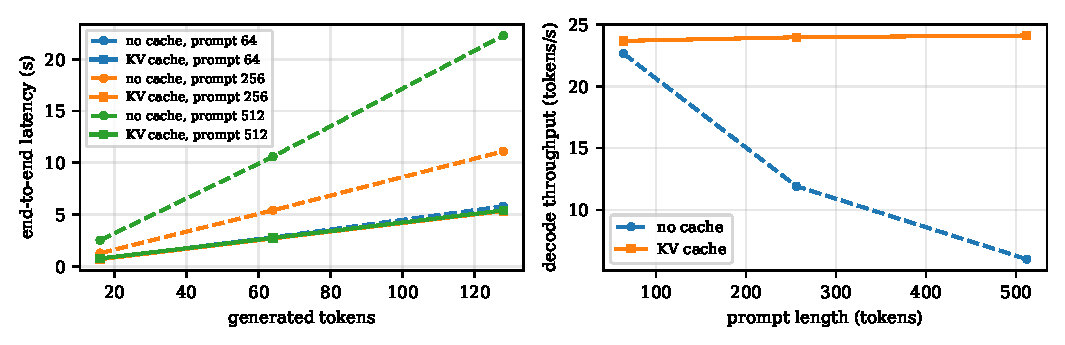
\includegraphics[width=0.82\textwidth]{figures/kv_cache.pdf}
\caption{Left: latency vs.\ generated tokens. Right: decode throughput vs.\ prompt length (T4, fp16). Uncached throughput collapses with context; cached throughput is flat.}
\label{fig:kv}
\end{figure*}

\subsection{Tiled Online-Softmax Attention}
\textbf{Correctness.} 29 unit-test cases (prefill, single-token decode with offset, multi-token verification, ragged block sizes 7$\times$13 and 16$\times$16, non-causal, Tq$>$block) agree with the reference within $10^{-5}$. Scores of order $10^4$ remain finite, and changing future keys does not change earlier outputs. Against an fp64 ground truth (T=256, fp32 inputs) the maximum absolute errors are $9.8\times10^{-7}$ (reference), $1.9\times10^{-6}$ (tiled) and $1.1\times10^{-6}$ (SDPA). On the T4 with fp16 inputs, errors against an fp32-accumulated reference are $\approx9.6\times10^{-4}$ for all kernels, dominated by rounding the output to fp16. Inside the full model, tiled and SDPA attention give token-identical outputs to the reference on all 10 validation prompts.

\textbf{Performance.} Fig.~\ref{fig:attn} shows the expected trade-off. At T=2048 (causal) the reference needs 576\,MiB of extra memory, because the $12\times T^2$ fp32 score, exponent and probability matrices are materialised; tiling needs 43\,MiB (13$\times$ less) and grows linearly. However, tiling is 9$\times$ slower (174 vs.\ 20\,ms). Each 64$\times$64 tile is a separate Python-level iteration that launches several small kernels and re-reads $Q$, $m$, $\ell$ and $a$ from GPU memory. FlashAttention's advantage comes from fusing that loop into one kernel that keeps the tile statistics in on-chip SRAM. PyTorch's fused SDPA (2.6\,ms, 18.5\,MiB) shows what fusion buys. Our implementation demonstrates the algorithm and its memory behaviour, not the IO-aware kernel.

\begin{figure*}[t]
\centering
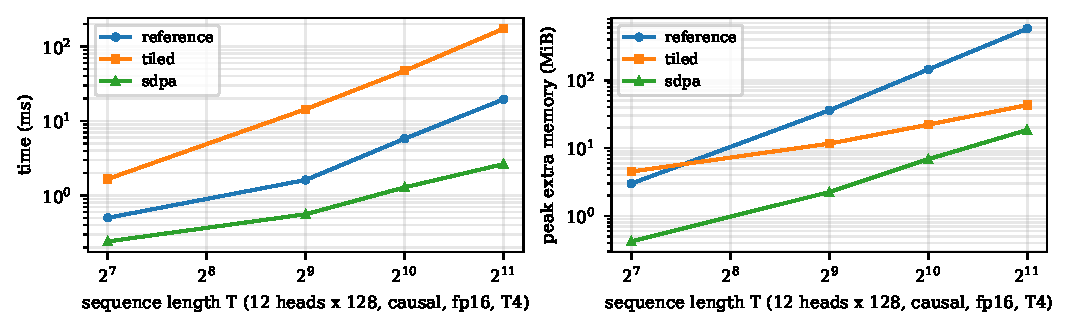
\includegraphics[width=0.82\textwidth]{figures/attention.pdf}
\caption{Attention kernels on a T4 (causal, fp16, 12 heads $\times$ 128). Tiled memory grows linearly instead of quadratically, but the unfused loop is slower than both the reference and fused SDPA.}
\label{fig:attn}
\end{figure*}

\subsection{Speculative Decoding}
The output of speculative decoding was token-identical to target-only greedy decoding in \textbf{all 72 GPU runs}, and in unit tests with a deliberately perturbed draft that forces rejections at $k\in\{1,3,5\}$. Table~\ref{tab:spec} and Fig.~\ref{fig:spec} summarise the T4 results. Fine-tuning the draft is decisive for this task: on criterion prompts the LoRA draft's proposals are accepted 97--98\% of the time, against 70--80\% for the base draft. The target then advances 3.8--4.0 tokens per pass at $k\ge4$, yet wall-clock speed-up is only 1.03--1.07$\times$. With the base draft, or on free text (acceptance 0.49--0.72), speculative decoding is 11--36\% \emph{slower}. Its peak extra memory is 7\,MiB higher (two caches), plus 1\,GB for the draft weights.

The reason is the cost ratio. Speculative decoding pays off when a draft step is much cheaper than a target step. On a T4 at batch 1 both models are launch-bound: the 0.5B draft has 24 layers against the target's 28, so a draft step costs about 80\% of a target step even though it has a third of the parameters. On the laptop CPU, decoding is memory-bandwidth bound and step cost scales with the bytes of weights read (2\,GB vs.\ 6.2\,GB in fp32). The same algorithm then gives \textbf{CPUSPEC} (Table~\ref{tab:spec}). The speed-up is a property of the hardware regime, not only of the acceptance rate.

\begin{table}[t]
\caption{Speculative decoding (mean over prompts; acceptance = accepted / drafted). T4 fp16 median of 3; CPU (i7-1255U, fp32) median of 2.}
\label{tab:spec}
\centering\footnotesize
\setlength{\tabcolsep}{3pt}
\begin{tabular}{@{}llcrrrr@{}}
\toprule
Prompts & Draft & $k$ & Accept & Tok/pass & Speed-up & Equal\\
\midrule
\multirow{4}{*}{Criterion (10)} & base 0.5B & 2 & 0.80 & 2.20 & 0.89 & 10/10\\
 & base 0.5B & 4 & 0.70 & 2.83 & 0.81 & 10/10\\
 & LoRA 0.5B & 2 & 0.97 & 2.59 & 1.04 & 10/10\\
 & LoRA 0.5B & 4 & 0.97 & 3.82 & \textbf{1.07} & 10/10\\
\midrule
\multirow{2}{*}{Free text (2)} & base 0.5B & 4 & 0.58 & 3.24 & 0.75 & 2/2\\
 & LoRA 0.5B & 4 & 0.61 & 3.33 & 0.77 & 2/2\\
\midrule
\multirow{2}{*}{CPU, criterion (4)} & base 0.5B & 4 & 0.61 & 2.61 & 0.98 & 4/4\
 & LoRA 0.5B & 4 & 1.00 & 3.85 & 	extbf{1.17} & 4/4\
\multirow{2}{*}{CPU, free text (2)} & base 0.5B & 4 & 0.59 & 3.28 & 1.24 & 2/2\
 & LoRA 0.5B & 4 & 0.61 & 3.33 & 	extbf{1.27} & 2/2\
\bottomrule
\end{tabular}
\end{table}

\begin{figure*}[t]
\centering
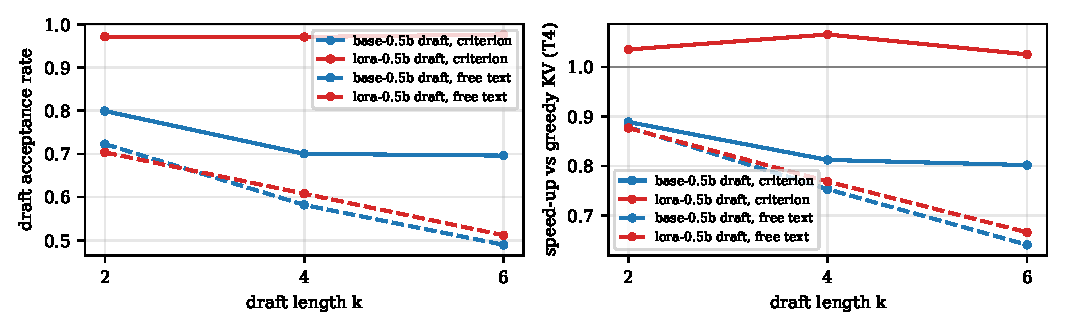
\includegraphics[width=0.82\textwidth]{figures/speculative.pdf}
\caption{Speculative decoding on a T4: acceptance rate and speed-up vs.\ draft length $k$. Only the fine-tuned draft on in-domain prompts beats greedy decoding.}
\label{fig:spec}
\end{figure*}

\subsection{Batched Screening on CPU}
We screened one validation patient against a 21-criterion trial (mean prompt 357 tokens, of which 238 are shared) on the laptop CPU, one run per method because each takes minutes. Sequential KV decoding took 255\,s. Sequential decoding with prefix reuse took 198\,s (1.29$	imes$): the shared note is prefilled once instead of 21 times. Batched decoding took 	extbf{61\,s (4.2$	imes$)}: 43.5\,s of prefill and 17.4\,s for 16 decoding steps. One step for all 21 rows costs about 1.1\,s, against 0.5\,s for a single row, because a CPU decoding step mostly streams the 6.2\,GB of fp32 weights from memory and that cost is shared across rows. All three methods produced identical outputs for all 21 criteria. We also tried bf16 weights (prefill 5$	imes$ slower: this CPU lacks native bf16 matrix units) and PyTorch dynamic int8 quantisation (slower, and 0/8 outputs matched fp32), and rejected both.

\subsection{Application}
Fig.~\ref{fig:app} shows the screening view and the inference lab. On the laptop, the application loads the merged model in about 15\,s, screens a 10-criterion trial in about 33\,s with batched decoding, and reproduces the evaluation script's predictions exactly (CPU fp32 vs.\ GPU fp16) on the checked examples. In a single lab run on one 369-token criterion prompt, uncached decoding took 76.8\,s, cached 13.1\,s, \code{generate()} 10.5\,s and speculative decoding with the LoRA draft 8.2\,s, all producing identical tokens.

APPFIG

\section{Limitations}
(1) Small data: 603 training annotations from 37 patients, with minority classes of 8--13 examples. The test split has no \emph{excluded} cases, so that class is untested and the 8-patient test set gives wide confidence intervals. (2) The model has not learned \emph{not included} and under-detects \emph{not applicable}; it also tends to read missing information as \emph{not excluded}, which in a real screening tool would wrongly keep ineligible patients in the pool. (3) Exclusion evidence recall is low (0.09). (4) Explanations are templated from the cited sentences. This is faithful by construction but not a reasoning trace, because the dataset's only free-text explanations are GPT-4 outputs, which we may not use. (5) Patient notes are short synthetic case descriptions, unlike real EHR text. (6) The tiled kernel is unfused and slow, and our decoders run at batch size 1 apart from per-patient batching. (7) The patient--trial outcome is a rule-based aggregation, not a validated eligibility decision. \textbf{The system is an educational screening prototype and must not be used for clinical enrollment.}

\section{Conclusion}
A 1.5B open model with LoRA, trained in 16 minutes on a free GPU, reaches 0.743 accuracy and 0.545 macro-F1 on held-out patients and cites the right note sentences about half the time (evidence micro-F1 0.508), up from 0.325/0.256/0.123 before fine-tuning. Re-implementing inference showed that each efficiency mechanism helps only in the regime it targets. KV caching helps once context is long enough to dominate launch overhead. Tiling saves memory but needs kernel fusion to save time. Speculative decoding needs an in-domain draft \emph{and} hardware where the draft is genuinely cheaper. Batching rows with different cache lengths was the largest practical win for interactive CPU screening. Future work: class-balanced training for the minority labels, an explicit penalty for citing nothing on exclusion criteria, and evaluation on real clinical notes.

\balance
\bibliographystyle{IEEEtran}
\bibliography{references}

\appendices
\section{Use of AI Assistants}
The implementation, experiments and this report were produced with the help of an AI coding assistant (Anthropic Claude, via Claude Code), which wrote most of the code and draft text under the author's direction. The author chose the overall approach, ran all training and benchmark jobs on Kaggle, checked results against the assignment rubric, and is responsible for every claim. All AI-written code was tested (36+ unit tests comparing the manual model, cache, attention kernels and speculative decoder with reference implementations), and all numbers in this report come from logged result files in the repository. Several issues were found and fixed through these checks: a hidden repetition penalty in the default generation configuration, a GPU out-of-memory configuration, library-version incompatibilities on Kaggle, and an attention ``fp64 ground truth'' that was silently computed in fp32. Hugging Face Transformers, PEFT, PyTorch and Gradio are used as libraries. TrialGPT code was not used.

\section{Reproducibility}
Code: \url{https://github.com/ibrahimmlk/trialsieve}. Adapters: \url{https://huggingface.co/ibrahimmlk/trialsieve-qwen2.5-1.5b-lora} and \url{https://huggingface.co/ibrahimmlk/trialsieve-qwen2.5-0.5b-draft-lora}. Split: \code{python scripts/make\_split.py} (manifest in \code{data/splits/split\_manifest.json}). Training and GPU evaluation: \code{notebooks/kaggle\_finetune.ipynb} and \code{notebooks/kaggle\_benchmarks\_final.ipynb}. Tests: \code{pytest tests}. Figures: \code{python scripts/make\_figures.py}. Application: \code{run\_app.bat}.

\end{document}
